\section{Adaptive AR Model Based Time-Frequency Estimation}

\begin{enumerate}[label=\alph*), leftmargin=*]

%% a)
\item
%

In figure \ref{fig:4_2_a_1} the non-stationary frequency, $f(n)$, and the corresponding phase, $\phi(n)$, time-series are provided.
Clearly, the frequency is time-variant, hence a model capable of capturing non-stationarity is required.

\begin{figure}[h]
    \centering
    \begin{subfigure}{0.49\textwidth}
        \centering
        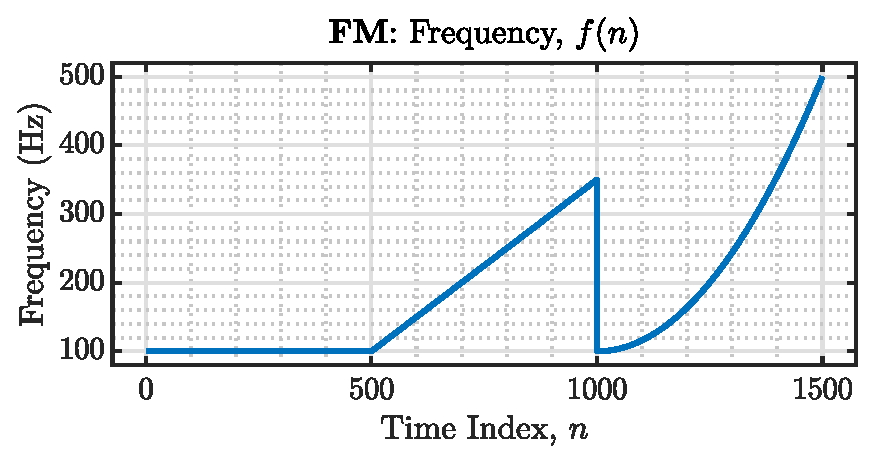
\includegraphics[height=1.5in]{report/widely-linear-filtering-and-adaptive-spectrum-estimation/adaptive-AR-model-based-time-frequency-estimation/assets/a/frequency}
    \end{subfigure}
    ~
    \begin{subfigure}{0.49\textwidth}
        \centering
        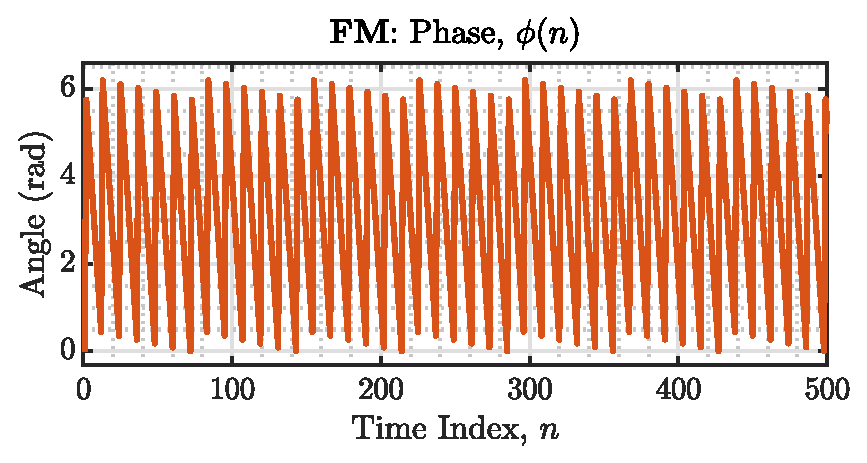
\includegraphics[height=1.5in]{report/widely-linear-filtering-and-adaptive-spectrum-estimation/adaptive-AR-model-based-time-frequency-estimation/assets/a/phase}
    \end{subfigure}
    \caption{FM: non-stationary frequency and phase time-series.}
    \label{fig:4_2_a_1}
\end{figure}

As expected, the static autoregressive order 1 model, AR(1), in figure \ref{fig:4_2_a_2}, fails to adapt to $f(n)$ over time, since a single peak is detected.
Increasing model order does not improve performance, since the static approach is incapable of dealing with non-stationary series, regardless the capacity of the model.

\begin{figure}[h]
    \centering
    \begin{subfigure}{0.32\textwidth}
        \centering
        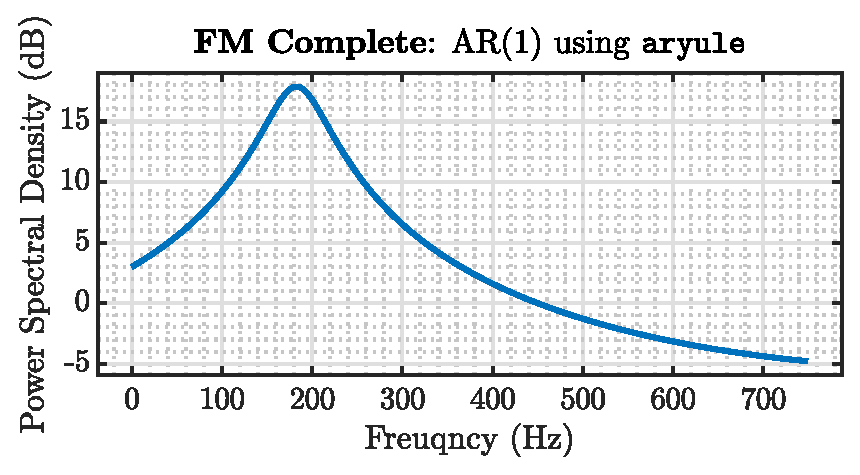
\includegraphics[height=1in]{report/widely-linear-filtering-and-adaptive-spectrum-estimation/adaptive-AR-model-based-time-frequency-estimation/assets/a/complete_aryule_1}
    \end{subfigure}
    ~
    \begin{subfigure}{0.32\textwidth}
        \centering
        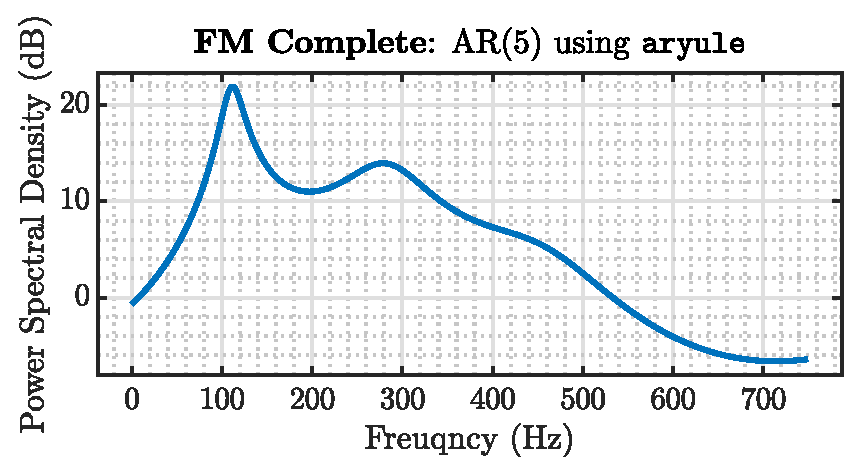
\includegraphics[height=1in]{report/widely-linear-filtering-and-adaptive-spectrum-estimation/adaptive-AR-model-based-time-frequency-estimation/assets/a/complete_aryule_5}
    \end{subfigure}
    ~
    \begin{subfigure}{0.32\textwidth}
        \centering
        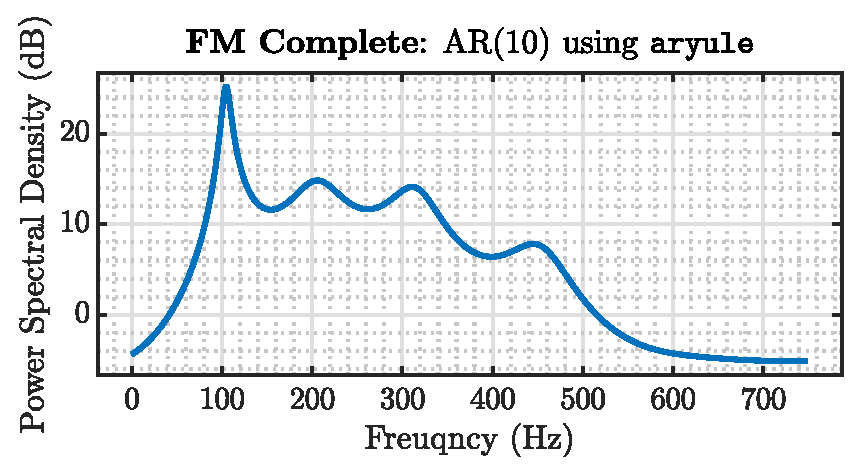
\includegraphics[height=1in]{report/widely-linear-filtering-and-adaptive-spectrum-estimation/adaptive-AR-model-based-time-frequency-estimation/assets/a/complete_aryule_10}
    \end{subfigure}
    \caption{FM: power spectrum and AR(p) models.}
    \label{fig:4_2_a_2}
\end{figure}

The frequency $f(n)$ is a branch function, a constant, a linear and a quadratic function, for different values of $n$. Splitting the signal into three series of segment length $N_{segment} = 500$,
we confirm that only the first segment (constant frequency $f = 100 Hz$ over time) can be adequately modelled, while the rest are failed due to their non-stationary nature.
Figure \ref{fig:4_2_a_2} illustrates the power spectral density estimates for the three segments.

\begin{figure}[h]
    \centering
    \begin{subfigure}{0.32\textwidth}
        \centering
        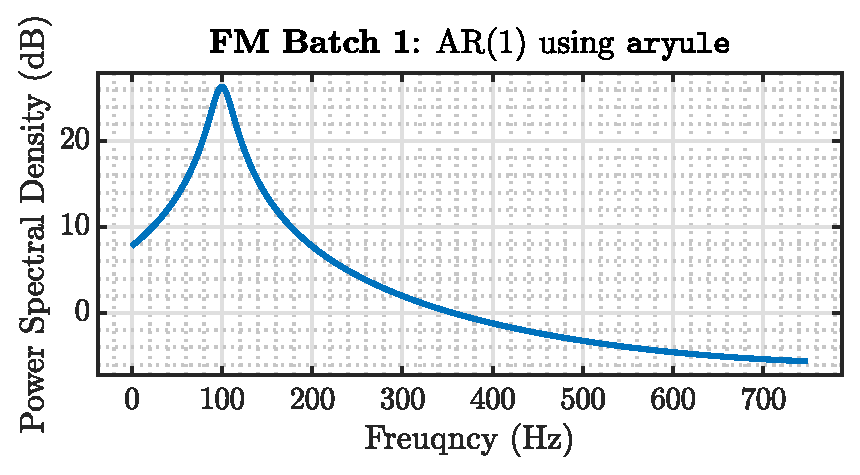
\includegraphics[height=1in]{report/widely-linear-filtering-and-adaptive-spectrum-estimation/adaptive-AR-model-based-time-frequency-estimation/assets/a/minibatch_1_aryule_1}
    \end{subfigure}
    ~
    \begin{subfigure}{0.32\textwidth}
        \centering
        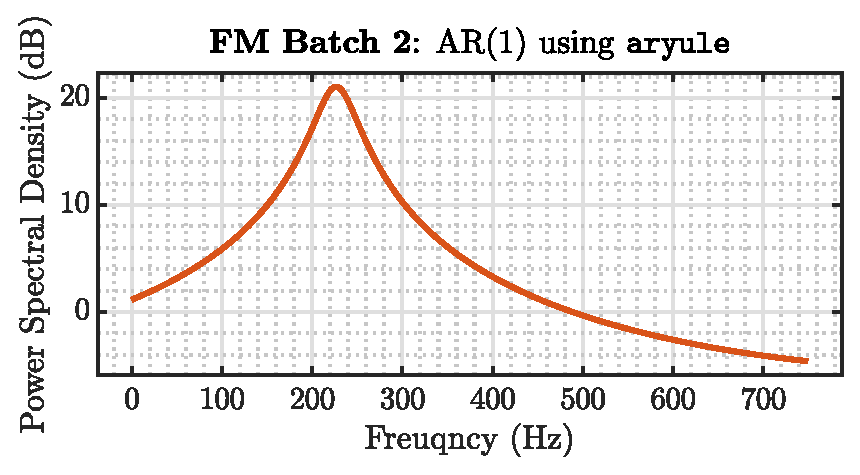
\includegraphics[height=1in]{report/widely-linear-filtering-and-adaptive-spectrum-estimation/adaptive-AR-model-based-time-frequency-estimation/assets/a/minibatch_2_aryule_1}
    \end{subfigure}
    ~
    \begin{subfigure}{0.32\textwidth}
        \centering
        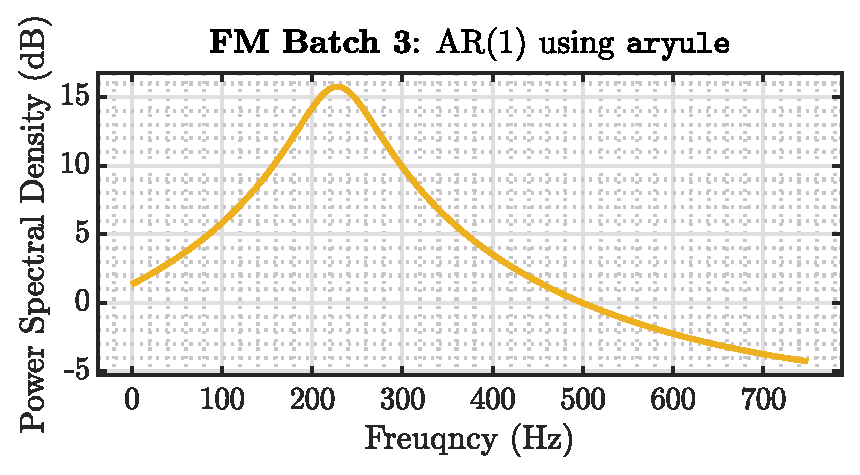
\includegraphics[height=1in]{report/widely-linear-filtering-and-adaptive-spectrum-estimation/adaptive-AR-model-based-time-frequency-estimation/assets/a/minibatch_3_aryule_1}
    \end{subfigure}
    \caption{FM: power spectrum of segments.}
    \label{fig:4_2_a_3}
\end{figure}

%% b)
\item
%

Having considered the deficiencies of the static AR models, a dynamic approach is now taken, using the CLMS algorithm, since the signal is complex.
Comparing figure \ref{fig:4_2_b}, the time-frequency spectrum plots, with the time-series $f(n)$ in figure \ref{fig:4_2_a_1}, we verify that the dynamic CLMS AR(1) model
enables the modelling of non-stationary processes.

The step-size $\mu$ of the CLMS filter is also varied, where for small values (i.e $\mu = 0.001$) the filter does not converge in-time to the correct frequencies,
while large $\mu$ values (i.e $\mu = 0.1$) lead to oscillations around the target value. This reflect once again the trade-off between convergence rate and steady-state error.
The wider bounds in the time-frequency plots (i.e for $\mu = 0.1$) the less certain the estimate is.

\begin{figure}[h]
    \centering
    \begin{subfigure}{0.49\textwidth}
        \centering
        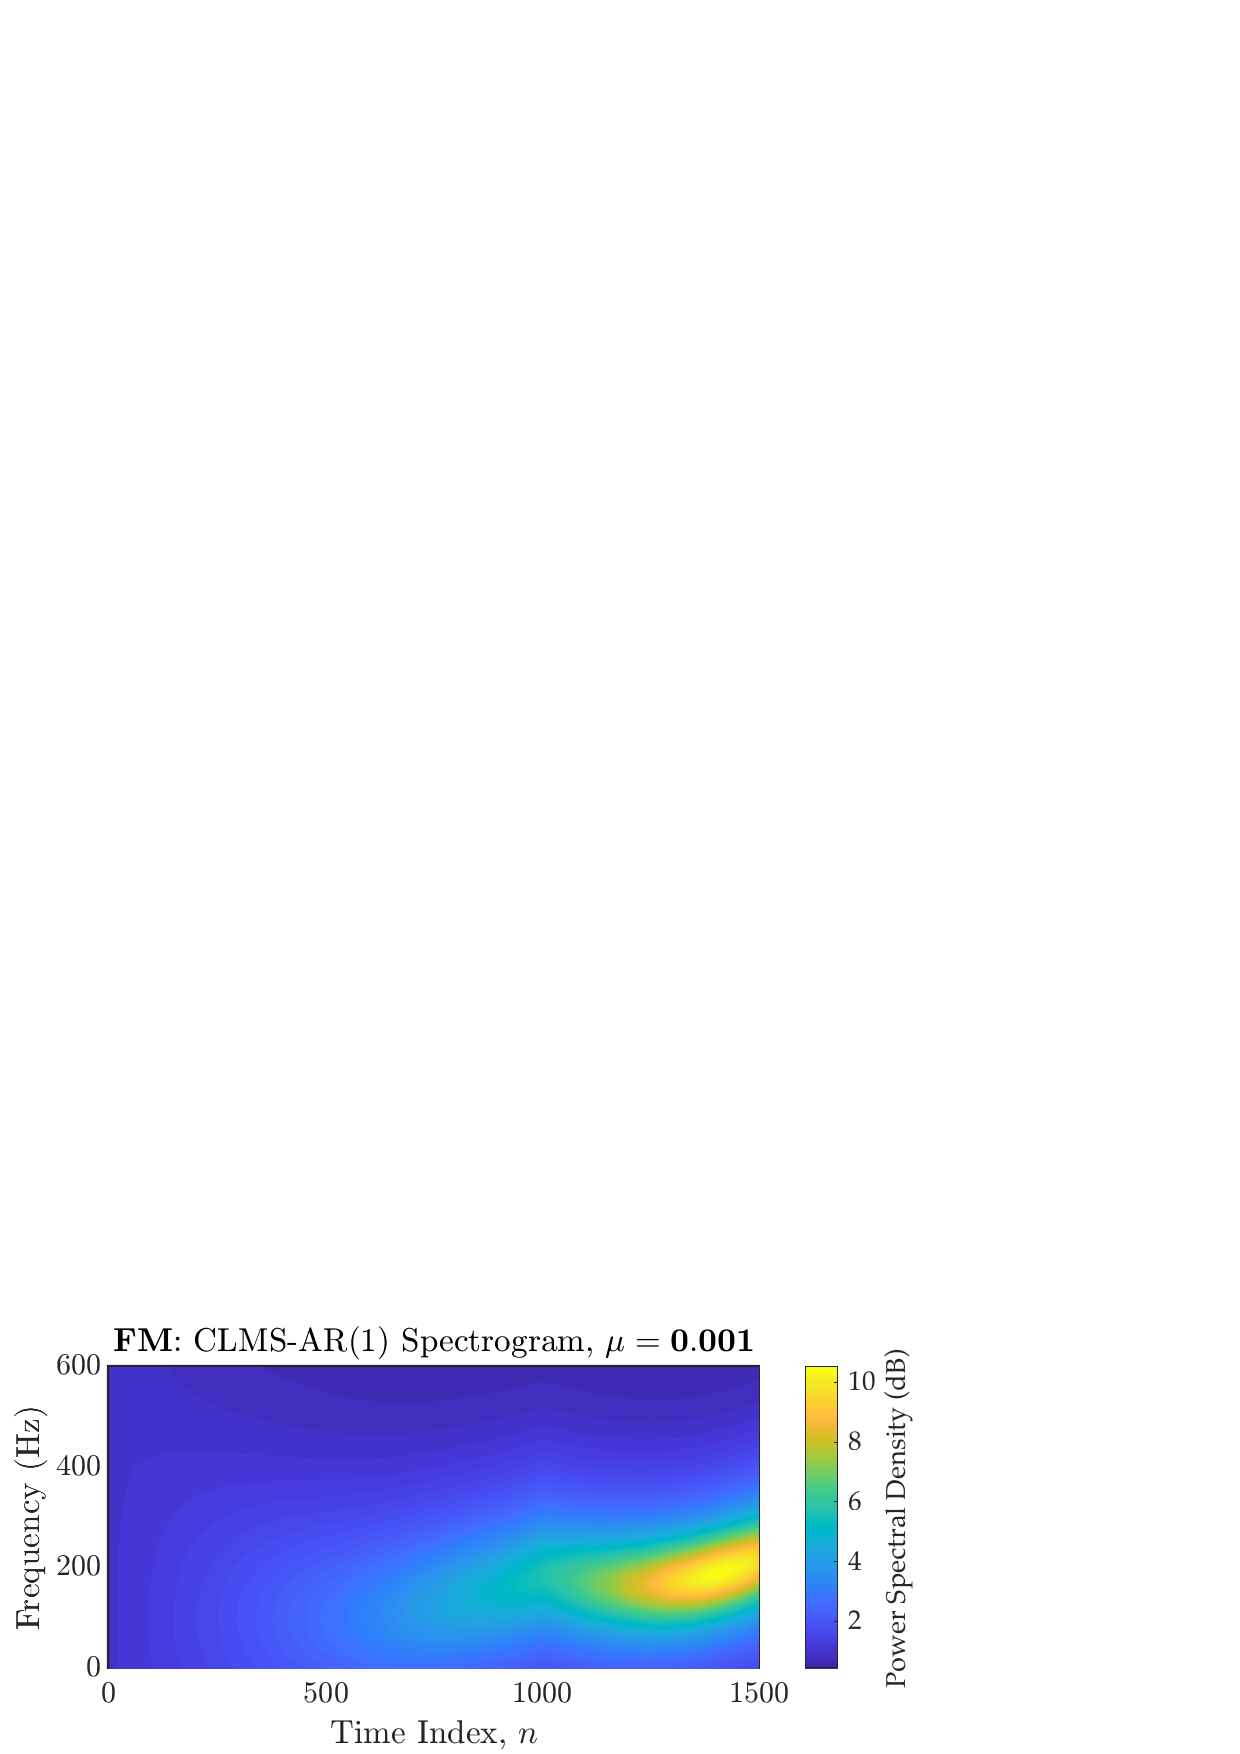
\includegraphics[height=1.5in]{{report/widely-linear-filtering-and-adaptive-spectrum-estimation/adaptive-AR-model-based-time-frequency-estimation/assets/b/time_frequency-mu_0.001}.pdf}
    \end{subfigure}
    ~
    \begin{subfigure}{0.49\textwidth}
        \centering
        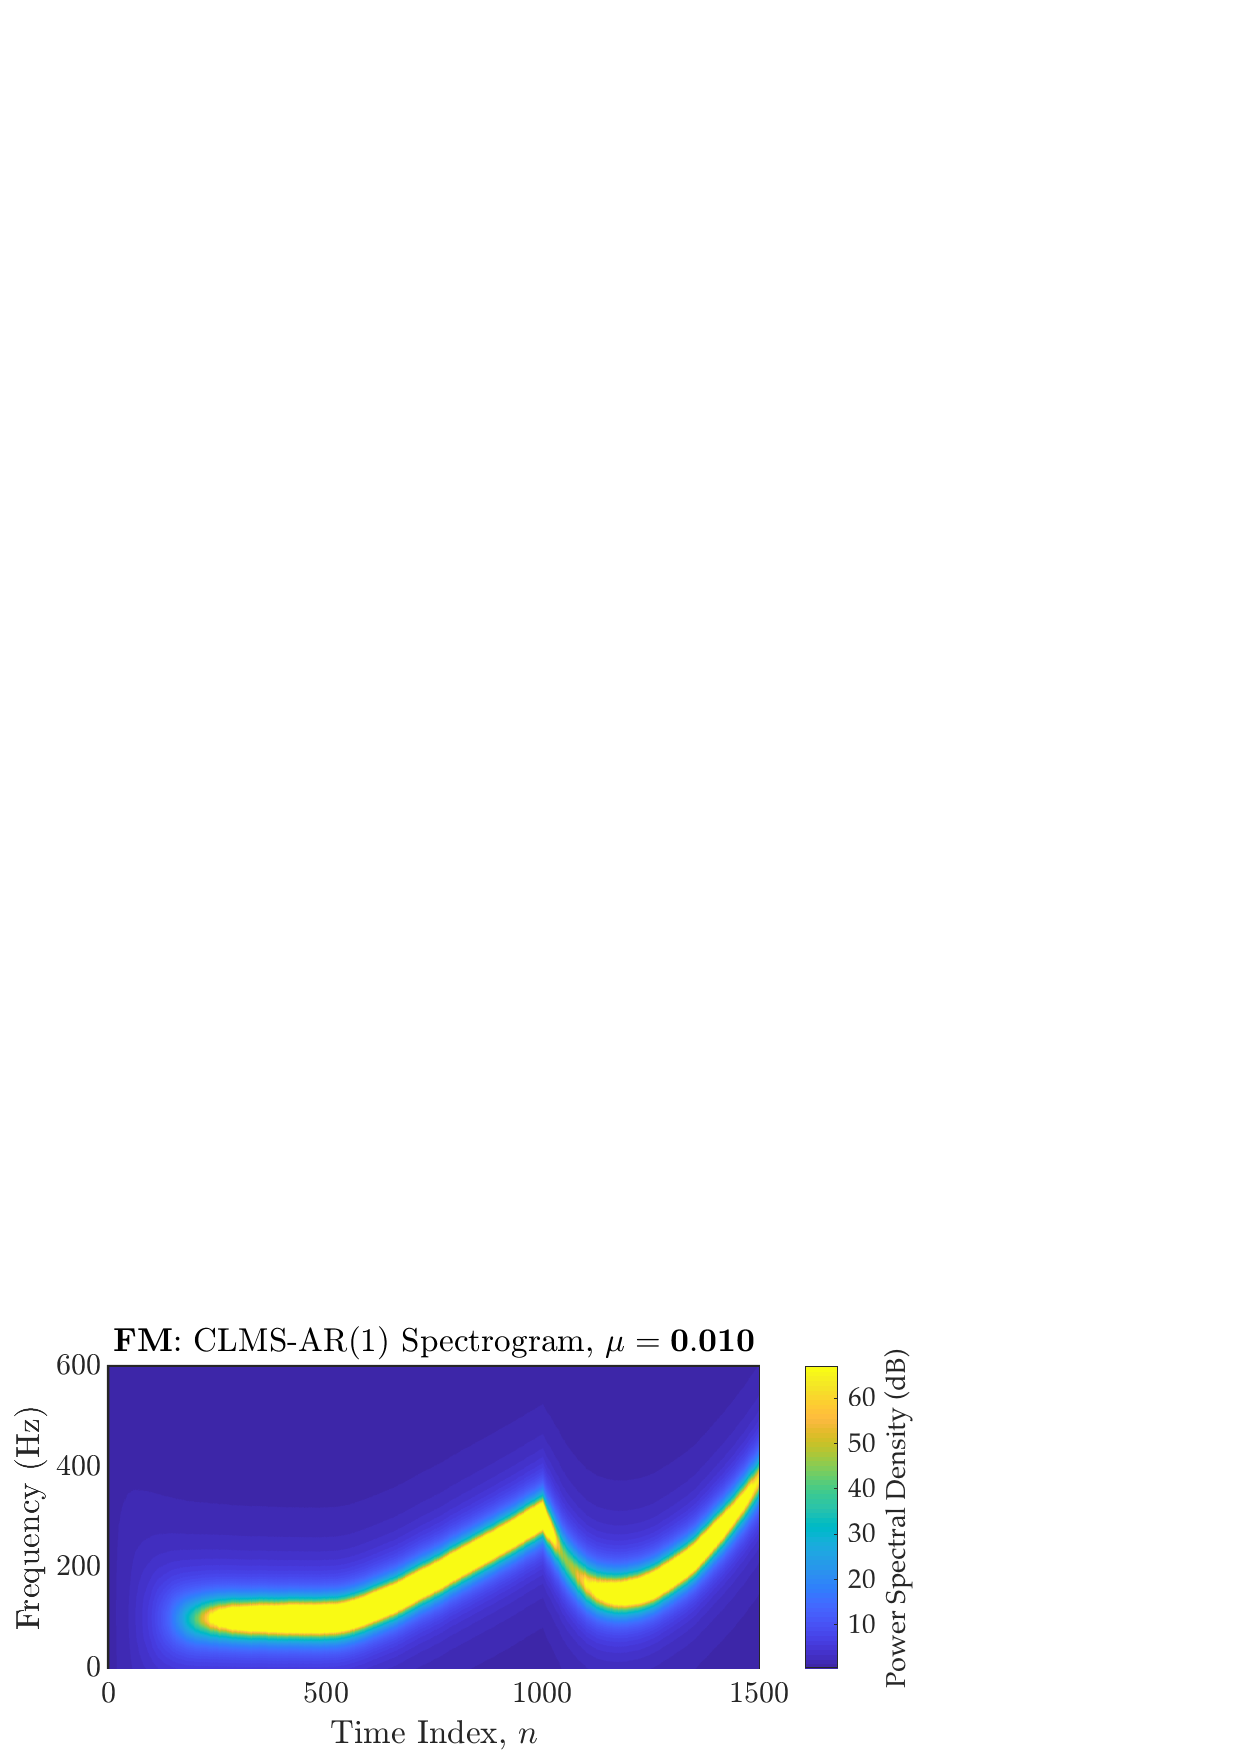
\includegraphics[height=1.5in]{{report/widely-linear-filtering-and-adaptive-spectrum-estimation/adaptive-AR-model-based-time-frequency-estimation/assets/b/time_frequency-mu_0.010}.pdf}
    \end{subfigure}
    ~
    ~
    \begin{subfigure}{0.49\textwidth}
        \centering
        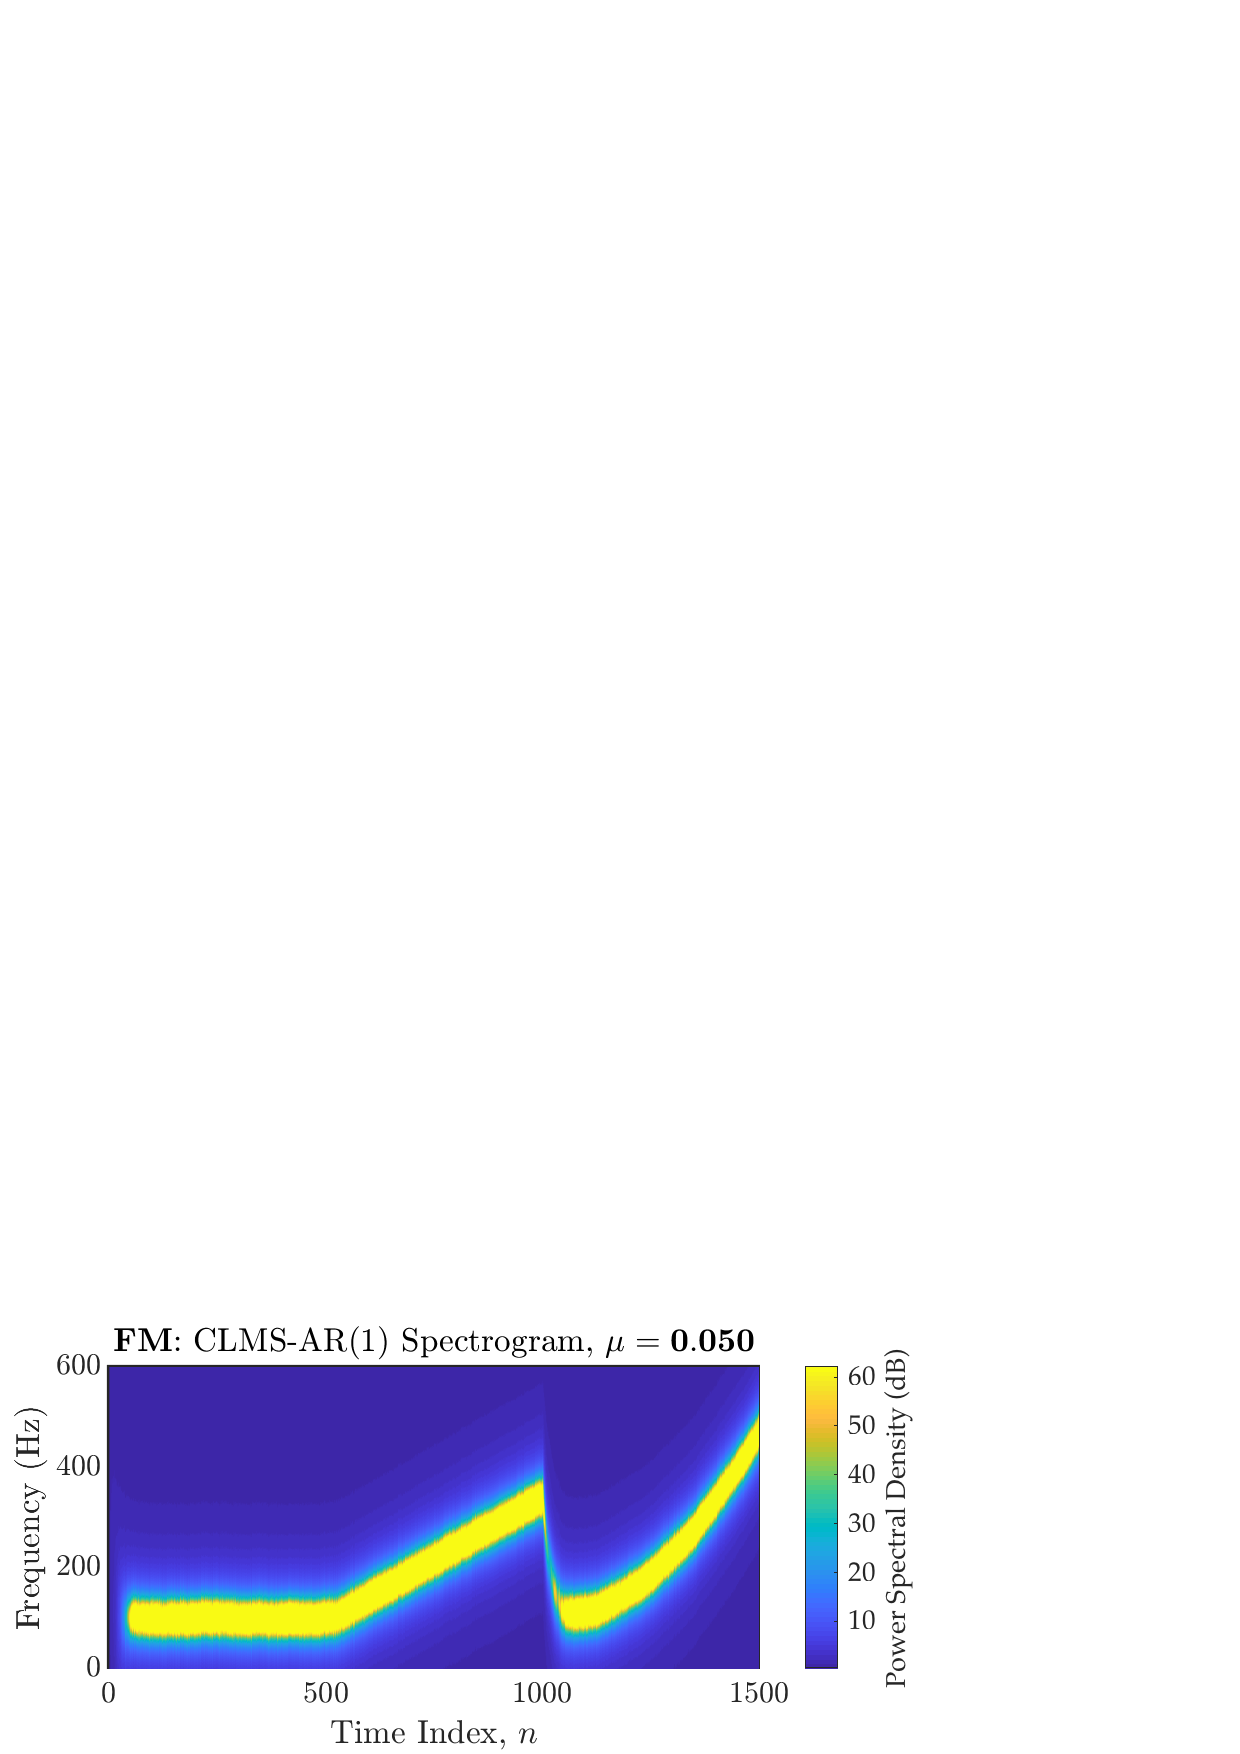
\includegraphics[height=1.5in]{{report/widely-linear-filtering-and-adaptive-spectrum-estimation/adaptive-AR-model-based-time-frequency-estimation/assets/b/time_frequency-mu_0.050}.pdf}
    \end{subfigure}
    ~
    \begin{subfigure}{0.49\textwidth}
        \centering
        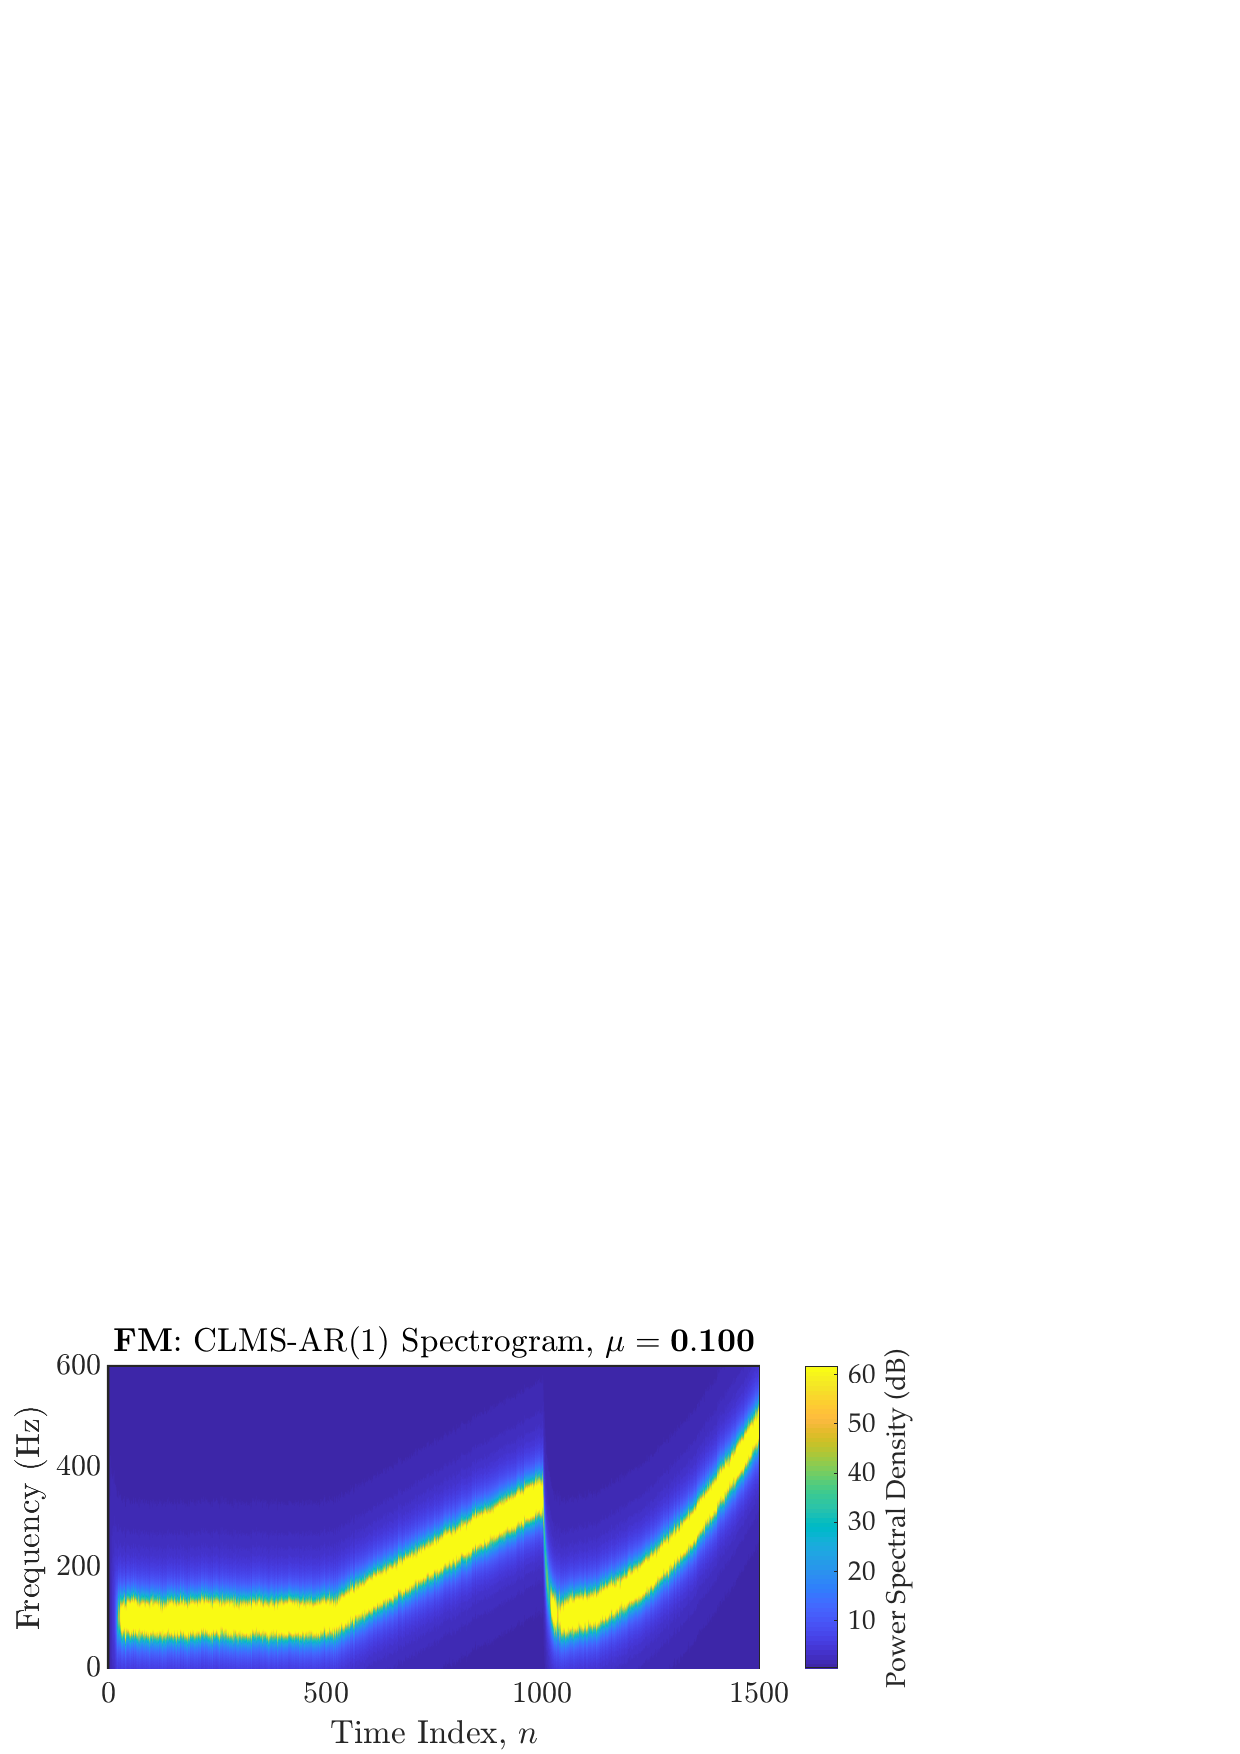
\includegraphics[height=1.5in]{{report/widely-linear-filtering-and-adaptive-spectrum-estimation/adaptive-AR-model-based-time-frequency-estimation/assets/b/time_frequency-mu_0.100}.pdf}
    \end{subfigure}
    \caption{FM: CLMS time-frequency plots.}
    \label{fig:4_2_b}
\end{figure}

%
\end{enumerate}